
\documentclass[tikz, border=1mm]{standalone}

\usepackage{amsmath}

\usepackage{tikz}

\usetikzlibrary{calc,angles,quotes,shapes.geometric}

\usepackage{tkz-euclide}

\begin{document}

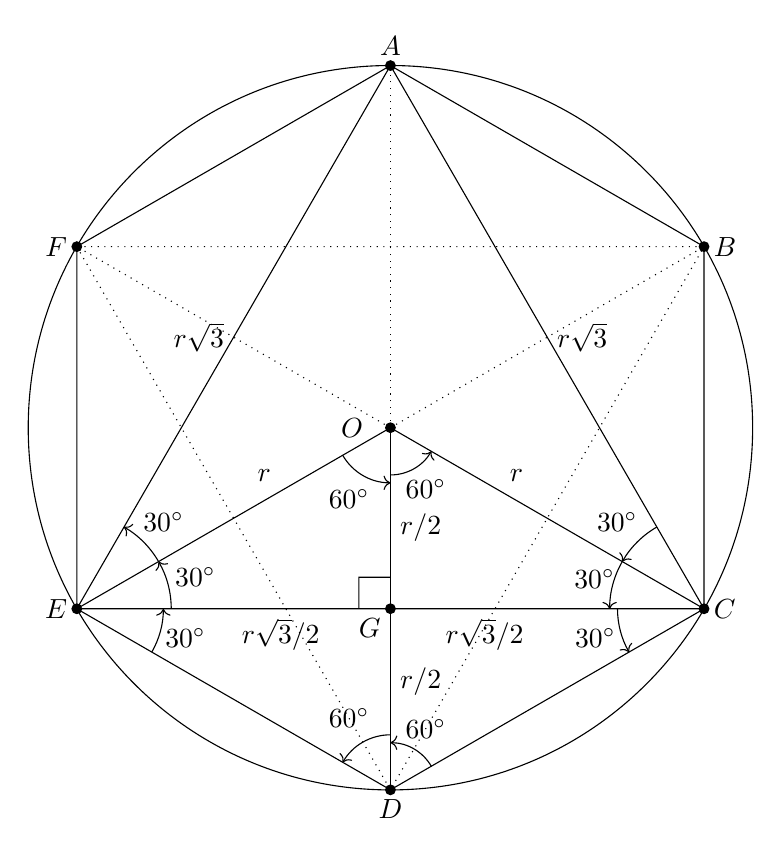
\begin{tikzpicture}[scale=2.3]

	% ---- parameters

	\def\numsides{6}
	\def\radius{2}
	\def\rotation{90}

	% ---- coordinates

	\coordinate (O) at (0,0);
	\foreach \i in {1,...,\numsides} {
		\coordinate (P\i) at ({360/\numsides*(\i-1)+\rotation}:\radius);
	}

	% cleaner with intersections
	%\coordinate (G) at (0,{-\radius/2});

	% ---- intersections

	\tkzInterLL(P1,P4)(P3,P5)\tkzGetPoint{G}

	% ---- circle

	\draw (O) circle (\radius);

	% ---- polygon

	\draw (P1) \foreach \i in {2,...,\numsides} { -- (P\i) } -- cycle;

	% ---- radiuses

	\draw[dotted] (O) -- (P1);
	\draw[dotted] (O) -- (P2);
	\draw (O) -- (P3);
	\draw (O) -- (P4);
	\draw (O) -- (P5);
	\draw[dotted] (O) -- (P6);

	% ---- hexagram

	\draw (P1) -- (P3) -- (P5) -- cycle;
	\draw[dotted] (P2) -- (P4) -- (P6) -- cycle;

	% ---- thick vertices

	\fill (O) circle (0.3mm);
	\fill (G) circle (0.3mm);
	\foreach \i in {1,...,\numsides} { \fill (P\i) circle (0.3mm); }

	% ---- vertices labels

	\node[label={[label distance=1.0mm]left:$O$}] at (O) {};

	\node[above] at (P1) {$A$};
	\node[right] at (P6) {$B$};
	\node[right] at (P5) {$C$};
	\node[below] at (P4) {$D$};
	\node[left] at (P3) {$E$};
	\node[left] at (P2) {$F$};

	\node[below left] at (G) {$G$};

	% ---- segments labels

	\node[below] at ($(P3)!0.65!(G)$) {$r \sqrt{3}/2$};
	\node[below] at ($(G)!0.3!(P5)$) {$r \sqrt{3}/2$};
	\node[left] at ($(P1)!0.5!(P3)$) {$r \sqrt{3}$};
	\node[right] at ($(P1)!0.5!(P5)$) {$r \sqrt{3}$};

	\node[right] at ($(O)!0.55!(G)$) {$r/2$};
	\node[right] at ($(G)!0.4!(P4)$) {$r/2$};

	\node[above left] at ($(O)!0.35!(P3)$) {$r$};
	\node[above right] at ($(O)!0.35!(P5)$) {$r$};

	% ---- angles labels

	\pic[draw, ->, "$60^\circ$", angle radius=0.7cm, angle eccentricity=1.5]
	{angle = P3--O--P4};

	\pic[draw, ->, "$60^\circ$", angle radius=0.6cm, angle eccentricity=1.5]
	{angle = P4--O--P5};

	\pic[draw, ->, "$60^\circ$", angle radius=0.7cm, angle eccentricity=1.5]
	{angle = O--P4--P3};

	\pic[draw, ->, "$60^\circ$", angle radius=0.6cm, angle eccentricity=1.5]
	{angle = P5--P4--O};

	\pic[draw, ->, "$30^\circ$", angle radius=1.2cm, angle eccentricity=1.3]
	{angle = G--P3--O};

	\pic[draw, ->, "$30^\circ$", angle radius=1.1cm, angle eccentricity=1.3]
	{angle = P4--P3--G};

	\pic[draw, ->, "$30^\circ$", angle radius=1.1cm, angle eccentricity=1.3]
	{angle = G--P5--P4};

	\pic[draw, ->, "$30^\circ$", angle radius=1.2cm, angle eccentricity=1.2]
	{angle = O--P5--G};

	\pic[draw, ->, "$30^\circ$", angle radius=1.2cm, angle eccentricity=1.3]
	{angle = O--P3--P1};

	\pic[draw, ->, "$30^\circ$", angle radius=1.2cm, angle eccentricity=1.3]
	{angle = P1--P5--O};

	% ---- right angles markers

	\pic[draw, angle radius=0.4cm, angle eccentricity=1]
	{right angle = O--G--P3};

\end{tikzpicture}

\end{document}
